\documentclass{article}
\usepackage[utf8]{inputenc}
\usepackage{polski}

\usepackage{bbm}
\usepackage{graphicx}    
\usepackage{caption}
\usepackage{subcaption}
\usepackage{epstopdf}
\usepackage{amsmath,amssymb,amsfonts,amsthm,mathtools}
\usepackage{hyperref}
\usepackage{url}
\usepackage{comment}
\usepackage[section]{placeins}
%\usepackage[polish]{babel}
\newtheorem{defi}{Definicja}
\newtheorem{twr}{Twierdzenie}


\author{Jan Mazur 281141}
\date{Wrocław, \today}
\title{\textbf{Obliczanie wartośći funkcji $\textrm{arctan}$ i $\textrm{arccot}$ } \\ Sprawozdanie do zadania P.1.4}

\begin{document}
\maketitle

\section{Wstęp}

Zadanie polega na obliczaniu wartośći funkcji $f(x) = \arctan(x)$ oraz\\ $f(x) = \textrm{arccot}(x)$, przy wykorzystaniu jedynie podstawowych działań arytmetycznych ( $+$, $-$, $*$, $/$ ).

\indent Przedstawię różne sposoby obliczania tych funkcji - szereg Taylora, szereg Eulera oraz nieskończony ułamek łańcuchowy. 
Dokładność wszystkich metod porównam z funkcjami biblioteczymi.
Wartośći funkcji  $f(x) = \textrm{arccot}(x)$ będę wyliczał za pomocą wzorów matematycznych z wcześniej wyliczonej wartośći funkcji $f(x) = \arctan(x)$

\indent Wszelkie obliczenia wykonane zostały wykonane przy użyciu języka programowania Julia w wersji 0.5.0, symulując 500-bitową mantysę zmiennopozycjnego zapisu liczb maszynowych.

\indent Kod źródłowy który został użyty do obliczeń, oraz do generowania wykresów znajduje się w pliku o rozszerzeniu .ipynb

\section{Uwarunkowanie zadania}
Przed przystąpieniem do jakichkolwiek obliczeń sprawdzam uwarunkowanie zadania. Wystarczy, że sprawdzę jak uwarunkowane jest obliczanie funkcji $\arctan(x)$, ponieważ wartośći funkcji $\textrm{arccot}(x)$ będę uzyskiwał odpowiednio przekształcając uzyskane wartości funkcji $arctan(x)$. Wskaźnik uwarunkowania wynosi:
\begin{equation}{\displaystyle cond(\mathbf {\arctan}(x) )}=\frac{x}{\left ( 1+x^{2} \right )\arctan x}\end{equation}

\begin{figure}[t]
	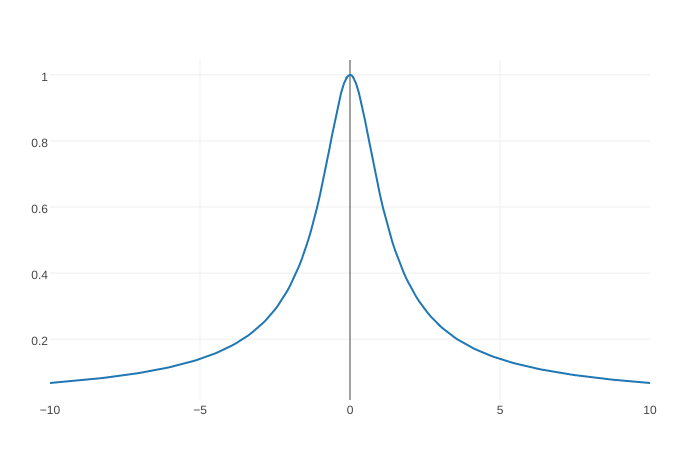
\includegraphics[width=\textwidth,scale=0.5]{cond.png}
	\caption{wskaźnik uwarunkowania}
	\label{wskaźnik uwarunkowania}
\end{figure}

\indent Maksimum globalne wskaźnika uwarunkowania wynosi 1 zatem można powiedzieć, że zadanie jest dobrze uwarunkowane.

\section{Szereg Taylora}
Pierwszy sposób obliczania wartości funkcji $\arctan(x)$ opiera się o rozwinięcie w szereg Taylora

\begin{equation}
\arctan(x)=x-{\frac {x^{3}}{3}}+{\frac {x^{5}}{5}}-{\frac {x^{7}}{7}}+\cdots =\sum _{n=0}^{\infty }{\frac {(-1)^{n}x^{2n+1}}{2n+1}}\,;\qquad |x|\leq 1\qquad 
\end{equation}

Szereg ten jest zbieżny tylko dla $x$ z przedziału $[-1,1]$.
Tabelka z iteracjami i błędami.

\section{Szereg Eulera}

Funkcję $\arctan$ rozwinąć można w inny szereg - szereg Eulera:

\begin{equation}
\arctan z=\sum _{n=0}^{\infty }{\frac {2^{2n}(n!)^{2}}{(2n+1)!}}\;{\frac {z^{2n+1}}{(1+z^{2})^{n+1}}}
\end{equation}

Szereg ten zbiega nieznacznie szybciej niż metoda poprzednia.
Jest zbieżny na całej prostej.
Tabelka z iteracjami i błędami.

\section{Nieskończony ułamek łańcuchowy}
Funkcja $\arctan$ może zostać zapisana również za pomocą nieskończonego ułamka łańcuchowego:

\begin{equation}
\arctan(x)={\frac {x}{1+{\cfrac {(1x)^{2}}{3+{\cfrac {(2x)^{2}}{5+{\cfrac {(3x)^{2}}{7+{\cfrac {(4x)^{2}}{9+\ddots }}}}}}}}}}
\end{equation}

Metoda ta okazuje się być najszybciej zbieżna ze wszystkich przeze mnie analizowanych. Jest zbieżna na całej prostej.

Tabelka z iteracjami i błędami.

\section{Zbijanie argumentu}

Opisane przeze mnie metody są dobrze zbieżnie w przedziale $[-1,1]$, natomiast poza tym przedziałem są zbieżne dużo wolniej, albo nawet wcale.
Aby zaradzić temu problemowi skorzystałem ze wzoru:

\begin{equation}
	{\begin{aligned}\arctan(x)&=2\arctan \left({\frac {x}{1+{\sqrt {1+x^{2}}}}}\right)\end{aligned}}
\end{equation}

Funkcja w argumencie $\arctan$ po prawej stronie ma zbiór wartości równy $(-1,1)$, więc wystarczy przed obliczeniami raz skorzystać z tego wzoru, aby znaleźć się w przedziale zbieżności opisanych metod.
Doświadczenia numeryczne pokazują jednak, że opłaca się zmniejszyć argument jak najbardziej, czyli skorzystać z tego wzoru kilkukrotnie.

\section{Obliczanie $\textrm{arccot}(x)$}
W celu obliczenia wartośći funkcji $\textrm{arccot}(x)$ skorystam ze wzoru:

\begin{equation}
\arctan \left({\frac {1}{x}}\right)=\operatorname {arccot}(x)\,,{\text{ if }}x>0
\end{equation}

Do obliczenia $\arctan(\frac{1}{x})$ użyję opisanych wcześniej metod.
Jakaś tabelka z wynikami i iteracjami.

\section{Porównanie zbieżności metod}
\subsection{$\arctan(x)$}
\FloatBarrier
	\begin{figure}[]
		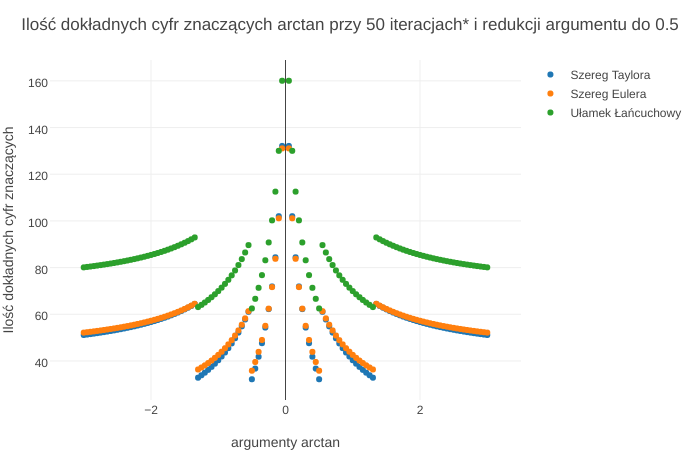
\includegraphics[width=\textwidth,scale=0.5]{atan_znaczace.png}
		\caption{porownanie ilości dokładnych cyfr znaczących}
		\label{wskaźnik uwarunkowania}
	\end{figure}
\FloatBarrier
\subsection{$\textrm{arccot}(x)$}
	\FloatBarrier
	\begin{figure}[]
		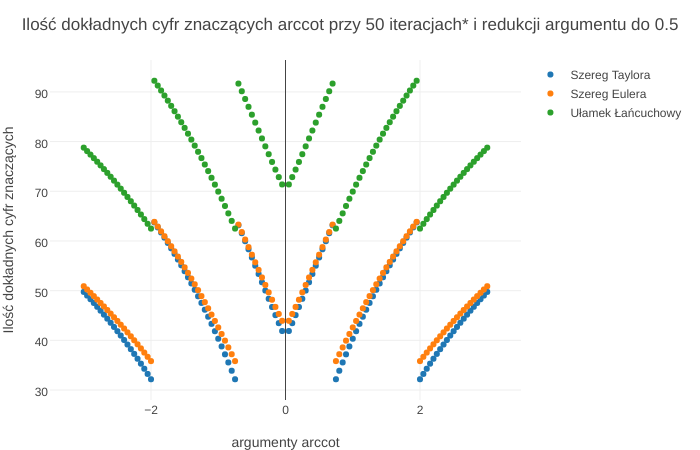
\includegraphics[width=\textwidth,scale=0.5]{acot_znaczace.png}
		\caption{porownanie ilości dokładnych cyfr znaczących}
		\label{wskaźnik uwarunkowania}
	\end{figure}
	\FloatBarrier
	
\section{Wnioski}
Bla bla bla Taylor najwolniej zbieżny i tylko w [-1,1]
, euler troche szybszy, ale zbieżny na całym R.
Nieskończony ułamek najszybciej zbieżny i zbieżny na całym R.
Bardzo opłaca się zbijanie argmentu do poziomu 0.1


\begin{thebibliography}{9}
	\itemsep2pt
	\bibitem{taylor} \url{http://mathworld.wolfram.com/EulersContinuedFraction.html}
	(ostatni dostęp do strony \today).
	
	\bibitem{fraction} \url{http://mathworld.wolfram.com/e.html}
	(ostatni dostęp do strony \today).
	
\end{thebibliography}

\end{document}